In questa sezione verrà discusso il modo in cui è stato possibile effettuare lo \textit{slicing} della rete al fine di differenziare il trattamento di diversi flussi. In questo caso particolare, sfruttando la stessa vista logica della rete utilizzata nella sezione precedente, facciamo in modo che lo \textit{slice} inferiore sia destinato al traffico normale e alla connessione di tutti gli host tra di loro, mentre lo \textit{slice} superiore sia destinato al traffico video. 
Per effettuare questa separazione, vengono implementati dei filtri sugli switch s1 ed s2. Gli switch s3 ed S4 controllano che effettivamente il flusso sia di tipo \textit{streaming video}, altrimenti non inoltrano il pacchetto ed interrompono il flusso. 
Non sono state apportate modifiche alla struttura della rete tramite Mininet, quindi di seguito vengono esposte le modifiche alla classe del controllore Ryu. 

\vspace{.3cm}

\begin{pythoncode}
@set_ev_cls(ofp_event.EventOFPSwitchFeatures, CONFIG_DISPATCHER)
def switch_features_handler(self, ev):
    datapath = ev.msg.datapath
    ofproto = datapath.ofproto
    parser = datapath.ofproto_parser
    dpid = datapath.id
    self.logger.info(f"[FEATURES HANDLER] dpid={dpid}")
    if dpid == 1:
        port_up, port_dw = 3, 4
        port_h1, port_h2 = 1, 2
        for host_port in [port_h1, port_h2]:
            match = parser.OFPMatch(
                in_port=host_port,
                eth_type=0x0800,
                ip_proto=17,
                udp_dst=UDP_PORT_STREAMING
            )
            actions = [parser.OFPActionOutput(port_up)]
            self.add_flow(datapath, priority=100, match=match, actions=actions)
    elif dpid == 2:
        port_up, port_dw = 1, 2
        port_h3, port_h4 = 3, 4
        for host_port in [port_h3, port_h4]:
            match = parser.OFPMatch(
                in_port=host_port,
                eth_type=0x0800,
                ip_proto=17,
                udp_dst=UDP_PORT_STREAMING
            )
            actions = [parser.OFPActionOutput(port_up)]
            self.add_flow(datapath, priority=100, match=match, actions=actions)
    elif dpid == 3:
        match = parser.OFPMatch(
            in_port=1, eth_type=0x0800, ip_proto=17, udp_dst=UDP_PORT_STREAMING
        )
        actions = [parser.OFPActionOutput(2)]
        self.add_flow(datapath, priority=100, match=match, actions=actions)
        match = parser.OFPMatch(
            in_port=2, eth_type=0x0800, ip_proto=17, udp_dst=UDP_PORT_STREAMING
        )
        actions = [parser.OFPActionOutput(1)]
        self.add_flow(datapath, priority=100, match=match, actions=actions)
    elif dpid == 4:
        match = parser.OFPMatch(in_port=1)
        actions = [parser.OFPActionOutput(2)]
        self.add_flow(datapath, priority=1, match=match, actions=actions)
        match = parser.OFPMatch(in_port=2)
        actions = [parser.OFPActionOutput(1)]
        self.add_flow(datapath, priority=1, match=match, actions=actions)
    # regola di base -> manda pacchetto al controller
    match = parser.OFPMatch()
    actions = [parser.OFPActionOutput(ofproto.OFPP_CONTROLLER,
                                    ofproto.OFPCML_NO_BUFFER)]
    self.add_flow(datapath, priority=0, match=match, actions=actions)
\end{pythoncode}
\newpage
\noindent
Il service based forwarding è palesato nelle istruzioni che riguardano il match dei pacchetti sugli switch marginali, in cui viene definita la regola per cui se il pacchetto usa il protocollo IP/UPD sul porto 9999 (streaming video) viene mandato sempre sul path superiore, indipendentemente dal MAC dei dispositivi comunicanti. Gli switch s3 ed s4 invece si occupano in questo caso solo del forwarding bidirezionale nel caso in cui avvenga il match (IP/UDP sul porto 9999 per lo switch s3 e tutti gli altri pacchetti per lo switch s4).

\vspace{.3cm}
\begin{pythoncode}
@set_ev_cls(ofp_event.EventOFPPacketIn, MAIN_DISPATCHER)
def _packet_in_handler(self, ev):
    msg = ev.msg
    datapath = msg.datapath
    ofproto = datapath.ofproto
    parser = datapath.ofproto_parser
    dpid = datapath.id
    in_port = msg.match['in_port']

    pkt = packet.Packet(msg.data)
    eth = pkt.get_protocol(ethernet.ethernet)
    if eth is None:
        return
    dst = eth.dst
    src = eth.src
    self.mac_to_port.setdefault(dpid, {})

    self.mac_to_port[dpid][src] = in_port

    # dest mac conosciuto 
    if dst in self.mac_to_port[dpid]:
        out_port = self.mac_to_port[dpid][dst]
        actions = [parser.OFPActionOutput(out_port)]
    else:
        host_ports = {
            1: {1,2}, # [dpid] -> [h*,h*]
            2: {3,4}, 
            3: set(), # core UP
            4: set() # core down
        }

        interswitch_links = {
            1: {4}, # [dpid] -> down path 
            2: {2},
        }

        actions = []
        for p in host_ports.get(dpid, set()):
            if p != in_port:
                actions.append(parser.OFPActionOutput(p))

        for p in interswitch_links.get(dpid, set()):
            if p != in_port:
                actions.append(parser.OFPActionOutput(p))

    if len(actions) == 1:
        match = parser.OFPMatch(in_port=in_port, eth_src=src, eth_dst=dst)
        self.add_flow(datapath, priority=1, match=match, actions=actions)

    out = parser.OFPPacketOut(
        datapath=datapath,
        buffer_id=msg.buffer_id,
        in_port=in_port,
        actions=actions,
        data=msg.data
    )
    datapath.send_msg(out)
\end{pythoncode}

\newpage
\noindent 
Questa funzione viene chiamata ogni volta che uno switch riceve un pacchetto, non trova nessun match e inoltra il pacchetto al controller.
Il controller estrae informazioni dal pacchetto e mantiene una tabella MAC per ogni switch, dove si trova l'associazione (MAC, port). 
Se la destinazione è già nota, questa viene utilizzata per l'inoltro diretto. Se la destinazione è ignota, viene inviato il pacchetto in flooding solo sulla rotta down.
Il test di questa implementazione è stato effettuato mediante i tool \textit{pingall} di Mininet, \textit{Wireshark} e \textit{iPerf} per la simulazione di traffico.

\begin{commandline}
\begin{verbatim}
mininet> pingall 
*** Ping: testing ping reachability

h1 -> h2 h3 h4 
h2 -> h1 h3 h4 
h3 -> h1 h2 h4 
h4 -> h1 h2 h3

*** Results: 0% dropped (12/12 received) 
\end{verbatim}
\end{commandline}

\noindent
La verifica con \textit{iperf} e \textit{wireshark} è stata efettuata configurando h1 come server e h4 come client. Lo scopo era evidenziare attraverso l'ascolto dei link collegati allo switch s3 che:
\begin{itemize}
    \item le politiche di service slicing sono state effettivamente applicate, infatti il traffico "video streaming" è visto solo sul path superiore e tutto l'altro traffico non è mai visto sul path superiore;
    \item la banda della rete dedicata è maggiore di quella della rete \textit{best effort} per costruzione, e quindi il traffico video gode di un throughput migliore.  
\end{itemize}

\begin{commandline}
\begin{verbatim}
mininet> h1 iperf -s -u -p 9999
mininet> h4 iperf -c h1 -u -p 9999 -b 10M -t 10
mininet> h1 killall iperf
mininet> h1 iperf -s -u -p 5000
mininet> h4 iperf -c h1 -u -p 5000 -b 1M -t 10
\end{verbatim}
\end{commandline}

\newpage
\begin{figure}[ht]
    \centering
    \setlength{\fboxrule}{.5pt} 
    \setlength{\fboxsep}{3pt} 
    \fbox{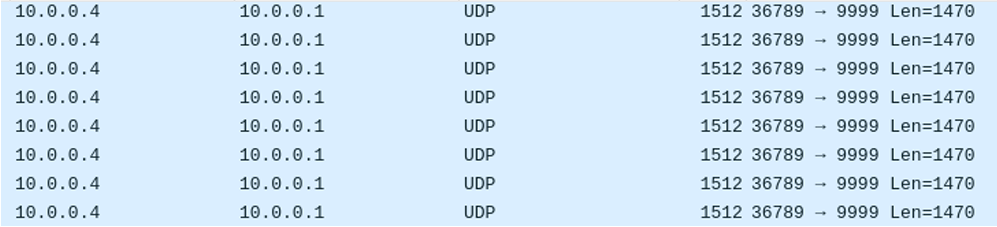
\includegraphics[width=0.9\textwidth]{img/S_whireshark_h4toh1_9999.png}}
    \label{img:h4toh1_9000}
\end{figure}

\begin{figure}[ht]
    \centering
    \setlength{\fboxrule}{.5pt} 
    \setlength{\fboxsep}{3pt} 
    \fbox{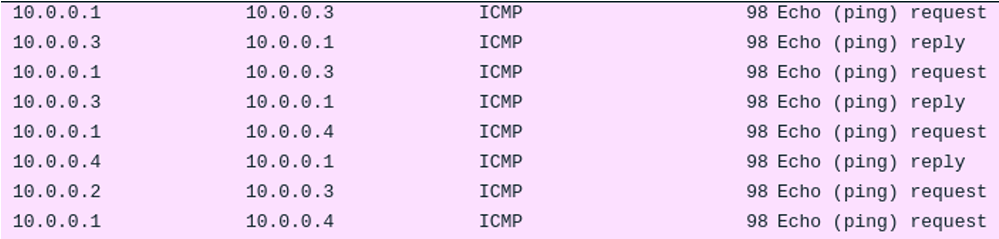
\includegraphics[width=0.9\textwidth]{img/down_traffic.png}}
    \label{img:down_traffic}
\end{figure}

\begin{figure}[ht]
    \centering
    \setlength{\fboxrule}{.5pt} 
    \setlength{\fboxsep}{3pt} 
    \fbox{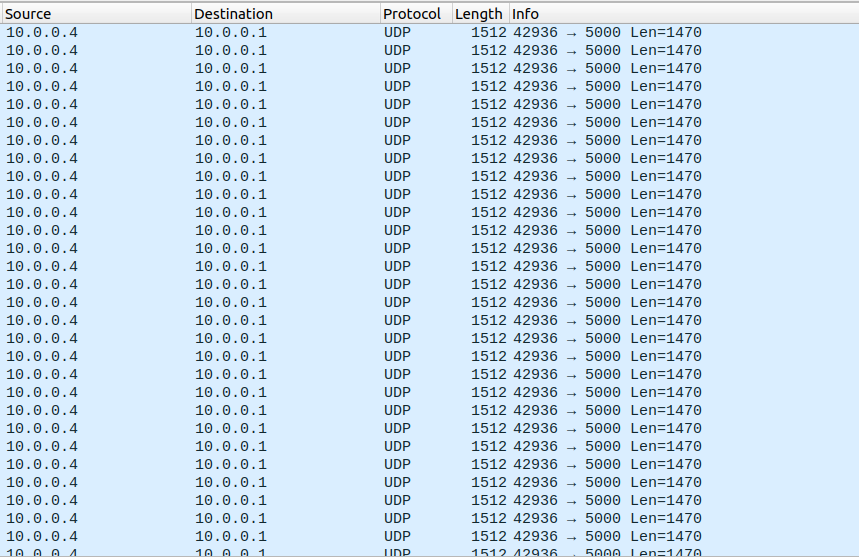
\includegraphics[width=0.9\textwidth]{img/S_wireshark_h4toh1_5000.png}}
    \label{img:h4toh1_5000}
\end{figure}

\begin{figure}[ht]
    \centering
    \setlength{\fboxrule}{.5pt} 
    \setlength{\fboxsep}{3pt} 
    \fbox{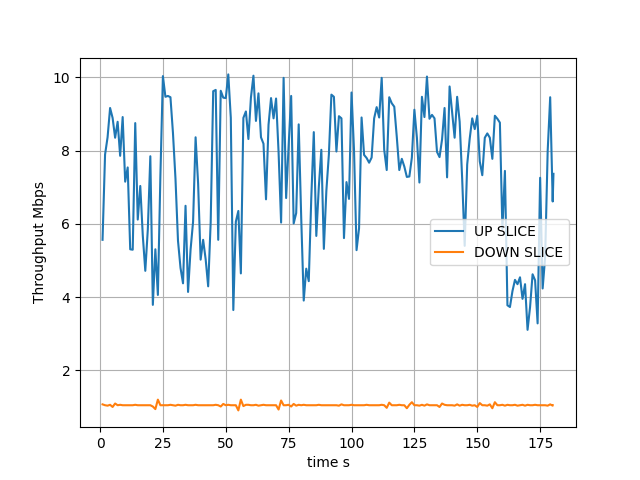
\includegraphics[width=0.9\textwidth]{img/throughput_compared.png}}
    \label{img:comparison}
\end{figure}


